% !TEX encoding = UTF-8 Unicode
\documentclass[11pt]{article} % use larger type; default would be 10pt

%%% PAGE DIMENSIONS
\usepackage{geometry} % to change the page dimensions
\geometry{a4paper} % or letterpaper (US) or a5paper or....


%%% PACKAGES
\usepackage[utf8]{inputenc} % set input encoding (not needed with XeLaTeX)
\usepackage{subfiles}
\usepackage{amssymb}
\usepackage{tabulary}
\usepackage{color, colortbl}
\usepackage{xcolor}


\usepackage{graphicx, wrapfig} % support the \includegraphics command and options

\DeclareGraphicsExtensions{.png,.jpg}
\graphicspath{{img/}{../img/}}
\usepackage{gensymb}
\usepackage{pdfpages}
\usepackage{standalone}
\usepackage{float}
\usepackage[toc,page]{appendix}

%%% Codes
\usepackage{listings}
\definecolor{Gray}{gray}{0.9}
\setlength{\parindent}{0em} 

\usepackage[breaklinks=true]{hyperref}


%%% HEADERS & FOOTERS
\usepackage{fancyhdr}	% This should be set AFTER setting up the page geometry
\pagestyle{fancy}	% options: empty , plain , fancy
\renewcommand{\headrulewidth}{0pt}	% customise te layout...
\lhead{}\chead{}\rhead{}
\lfoot{}\cfoot{\thepage}\rfoot{}

%%% END Article customizations

\begin{document}

\begin{titlepage}
    \begin{center}
        \vspace*{1cm}
        
        \Huge
        \textbf{WODSS}
        
        \vspace{0.5cm}
        \LARGE
        Event Planner
      
        \vspace{1.5cm}
        
        \textbf{Autoren: Andreas Gassmann, Jonas Frehner, Lukas Schönbächler}\\

		\vspace{1.5cm}        
                
        \vfill
        
       
        \vspace{0.8cm}
        
        
\includegraphics[width=0.4\textwidth]{title/fhnw}
        
        \Large
        FHNW\\
        Schweiz\\
        März 27, 2017
        
    \end{center}
\end{titlepage}

\begin{abstract}
Das Ziel dieser Arbeit ist die Entwicklung eines Tools welches das Managen von IT-Kolloquien der FHNW erlaubt.
\end{abstract}

\newpage
\tableofcontents
\newpage

\section{Prototyp}

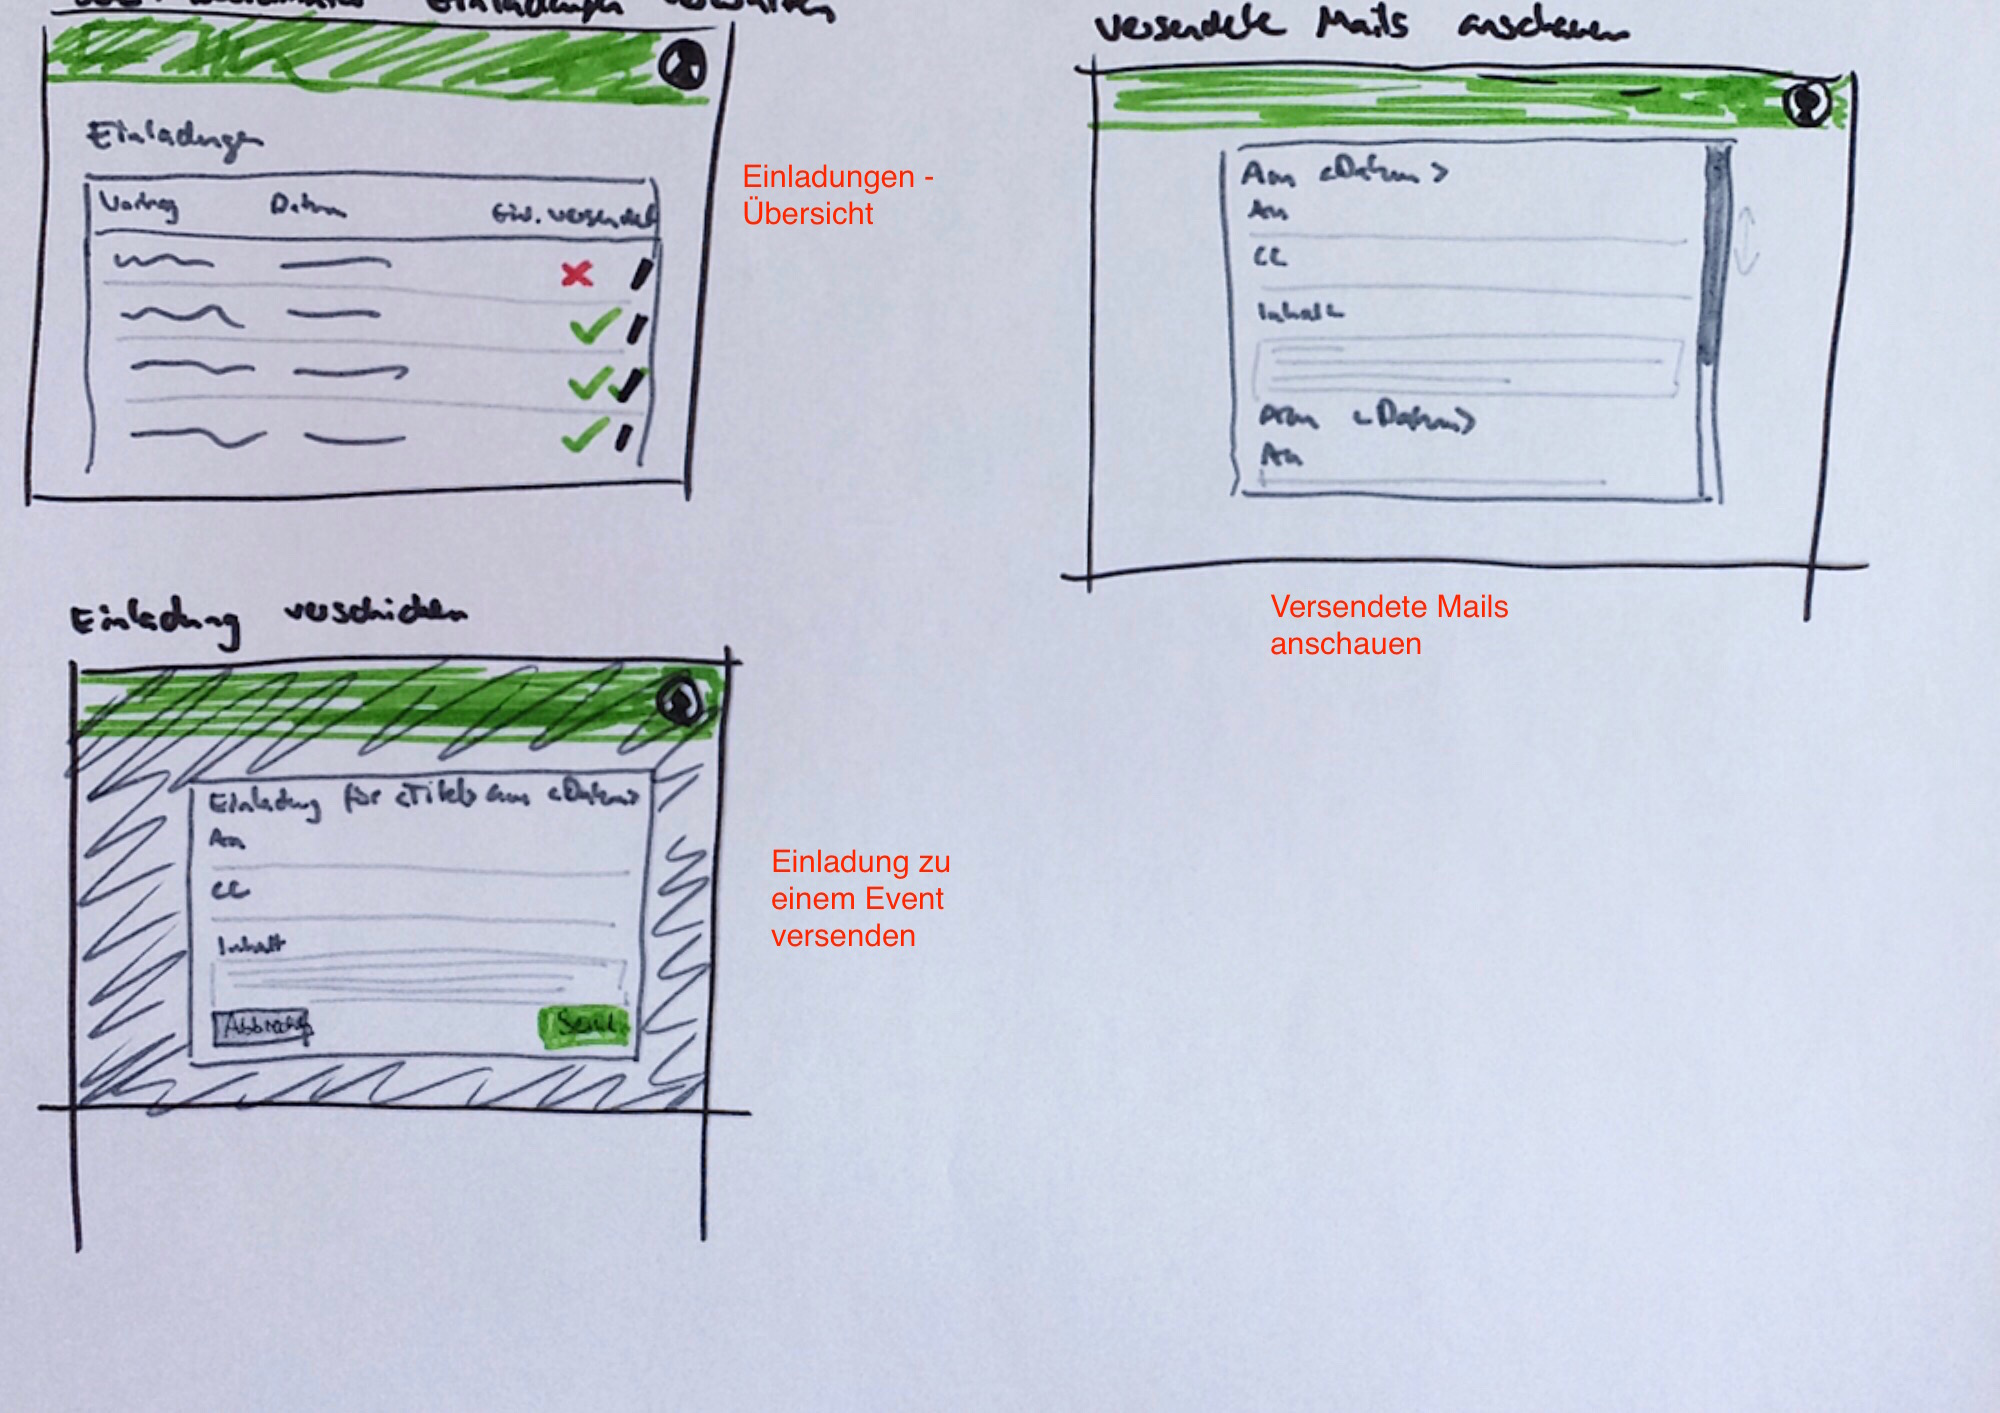
\includegraphics[width=0.8\textwidth]{prototyp/Einladungen}
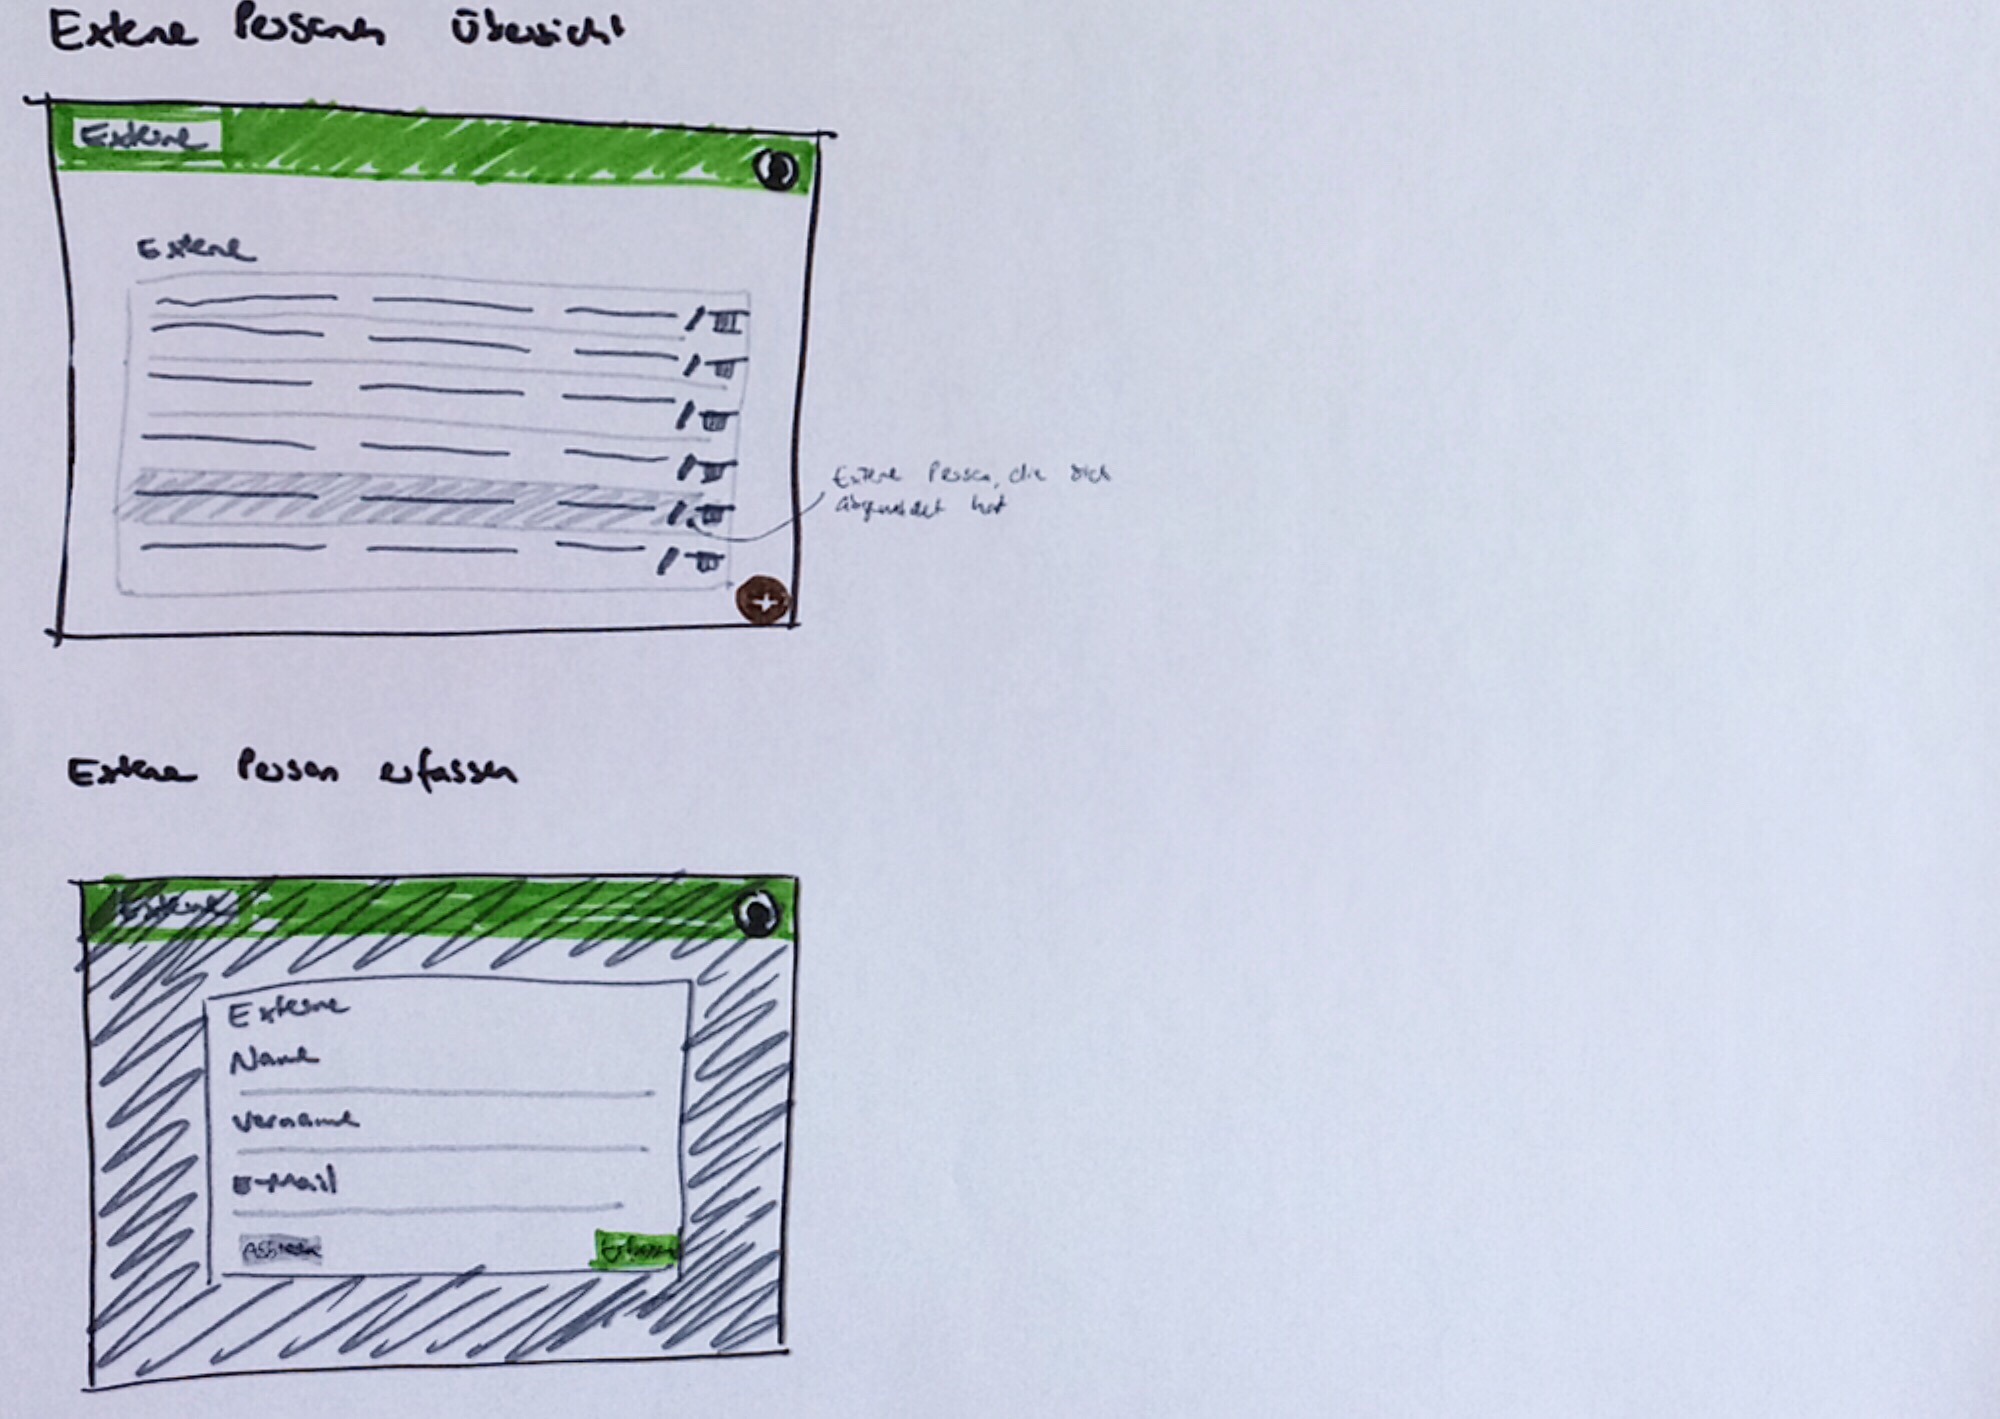
\includegraphics[width=0.8\textwidth]{prototyp/ExternePersonen}
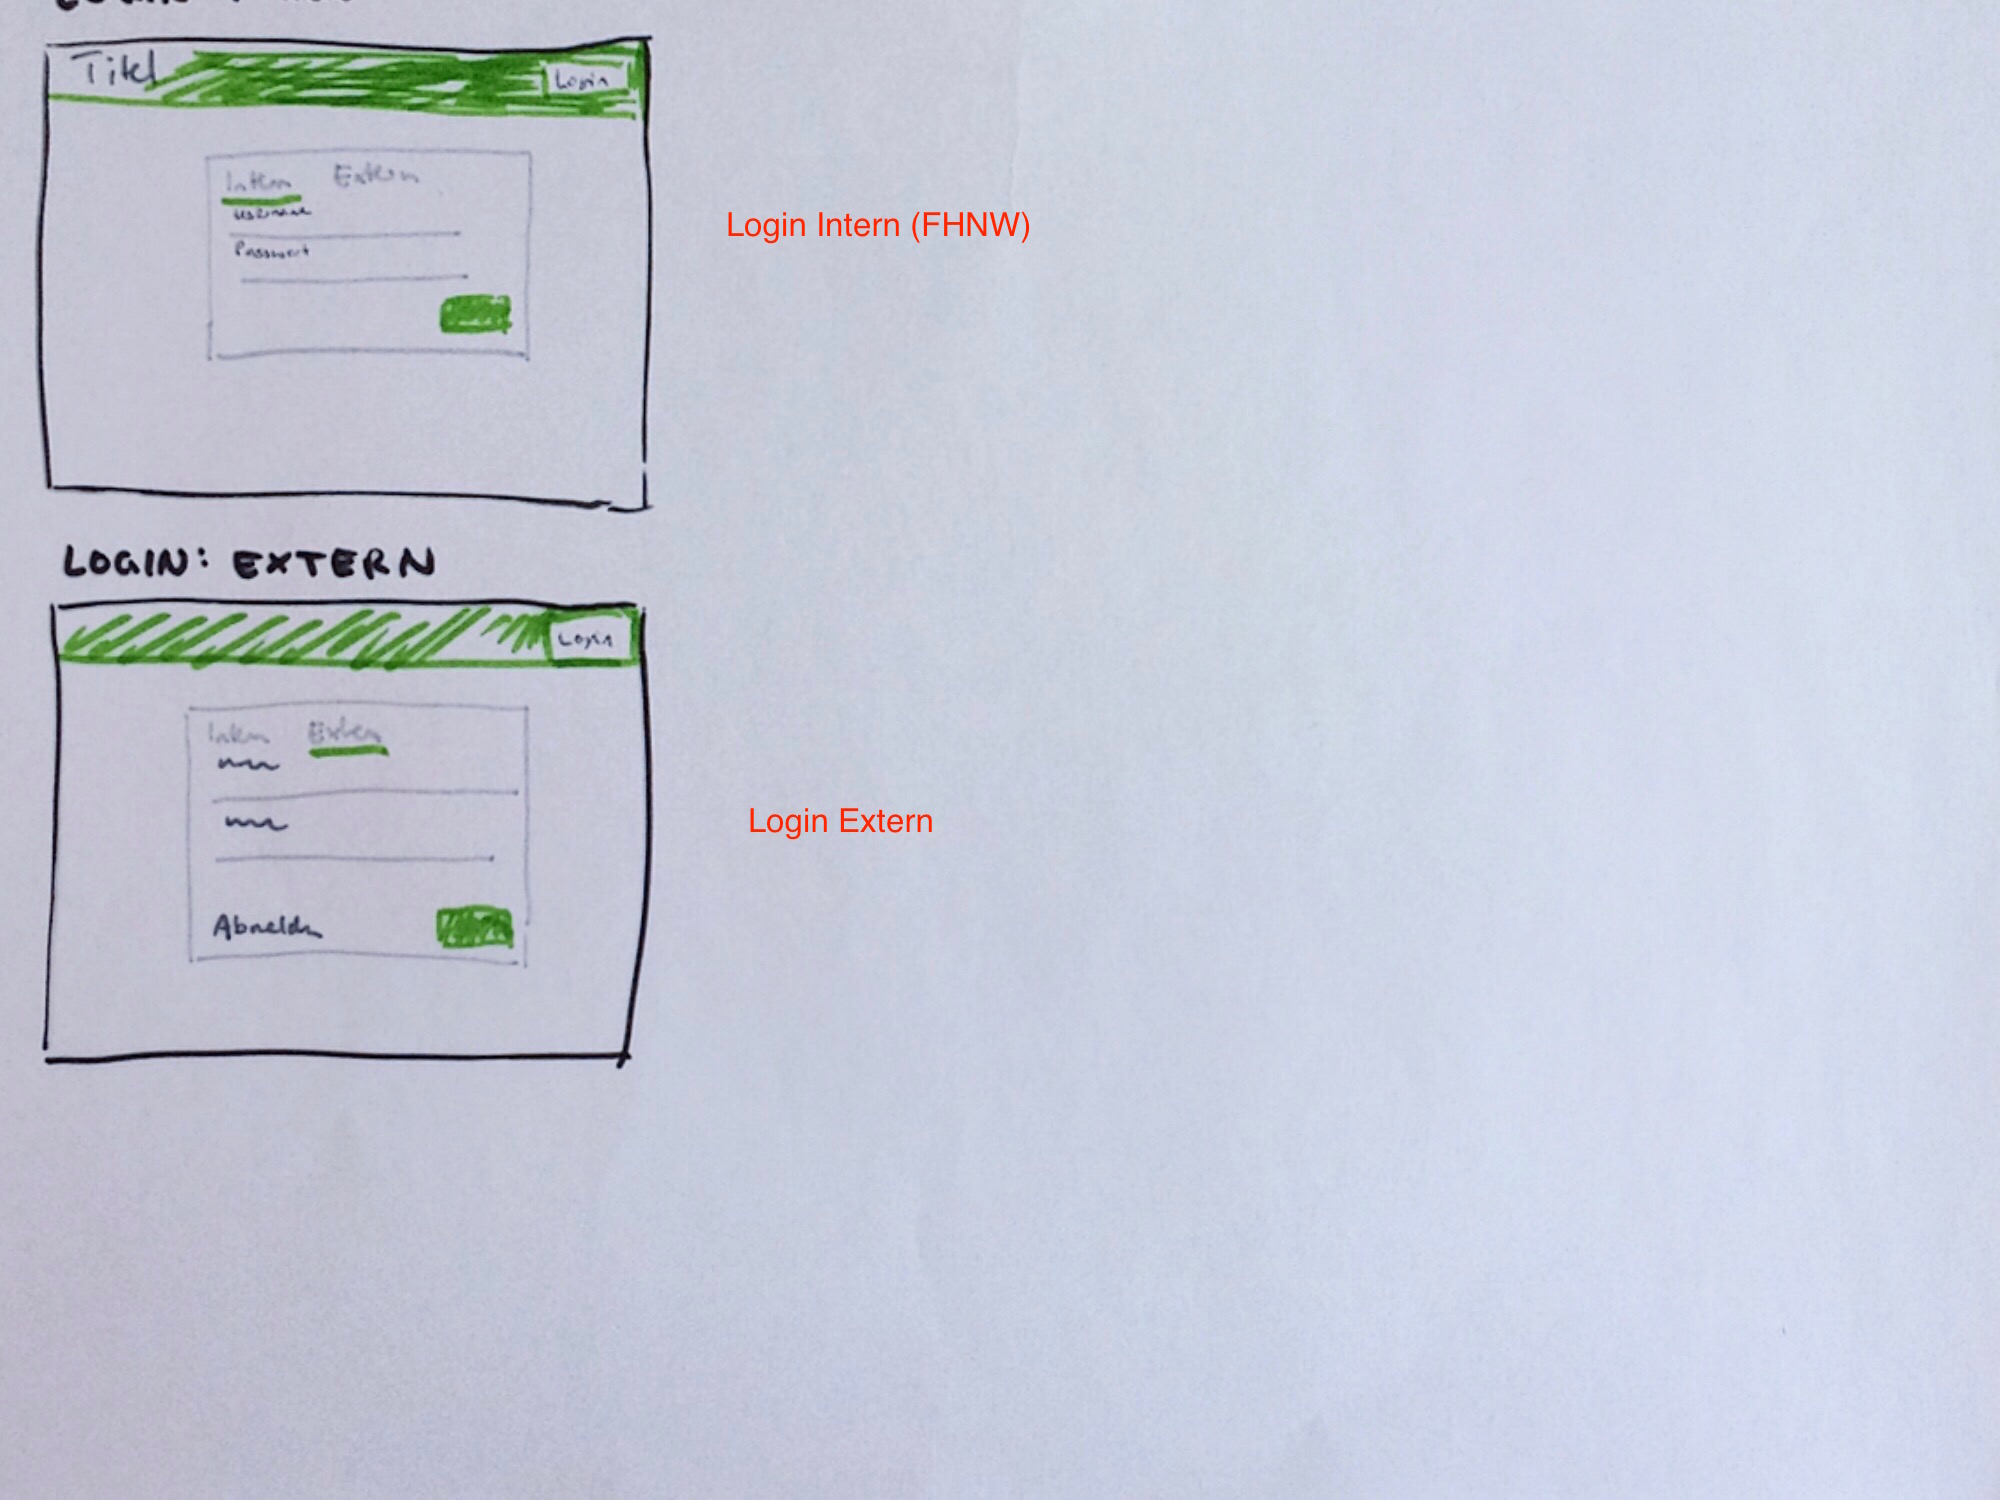
\includegraphics[width=0.8\textwidth]{prototyp/Login}
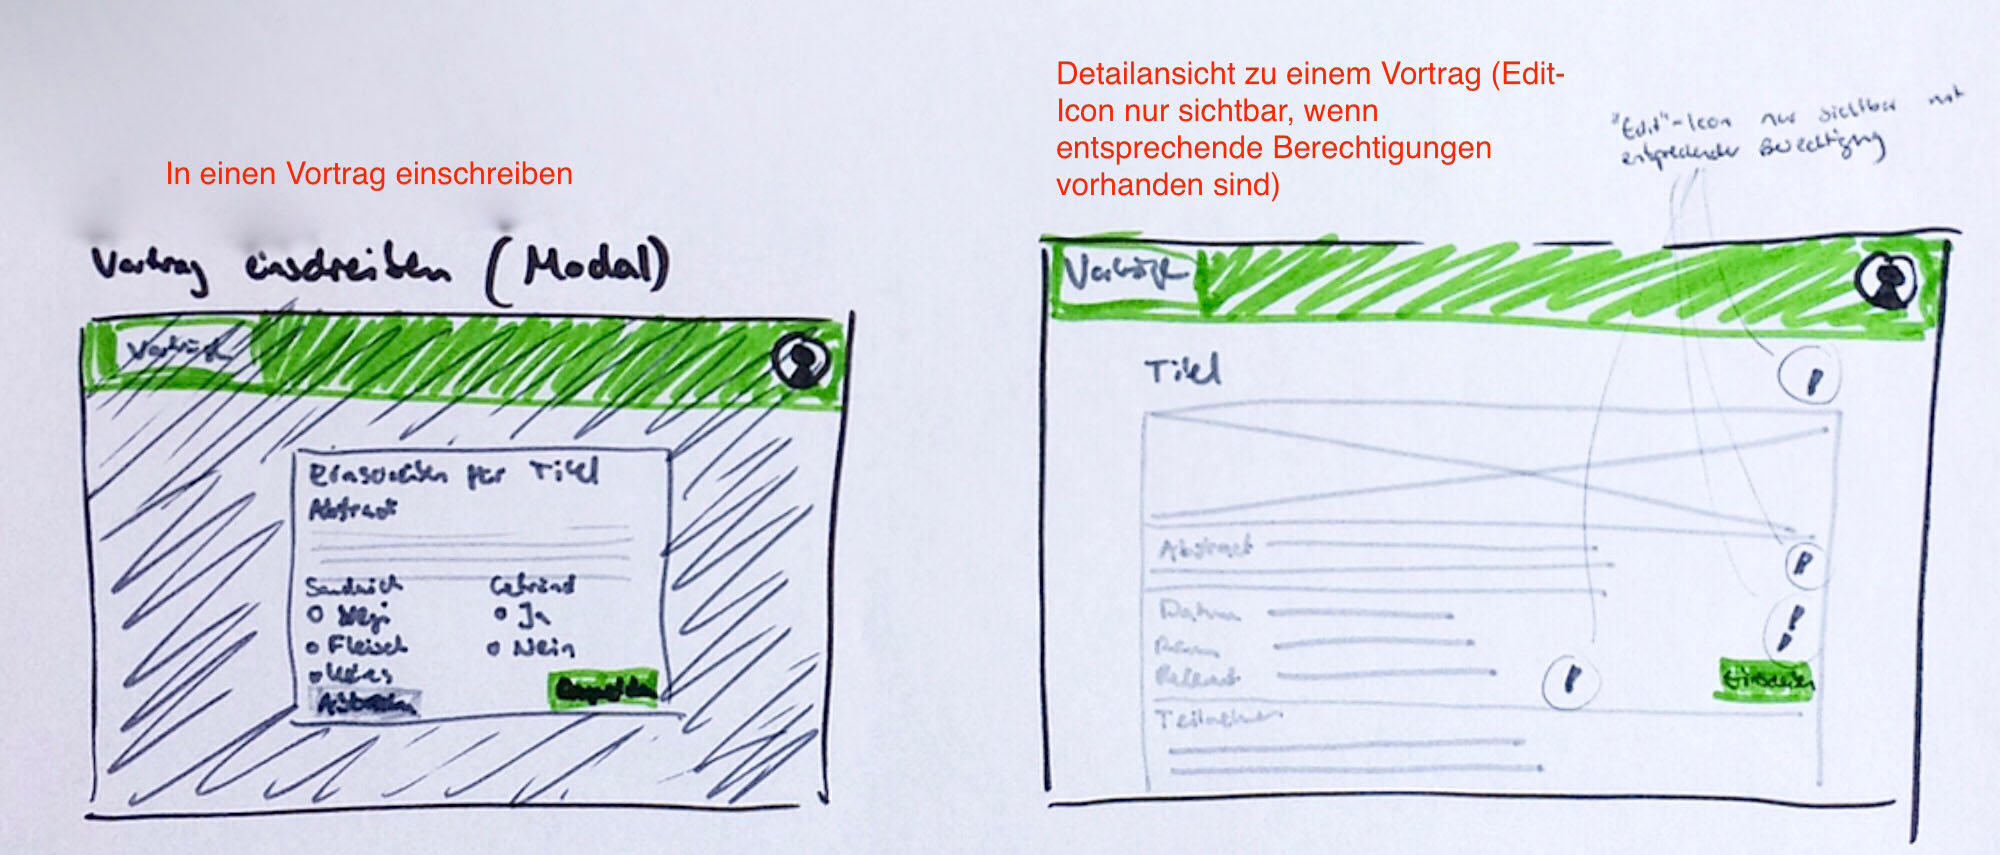
\includegraphics[width=0.8\textwidth]{prototyp/Vortrag}
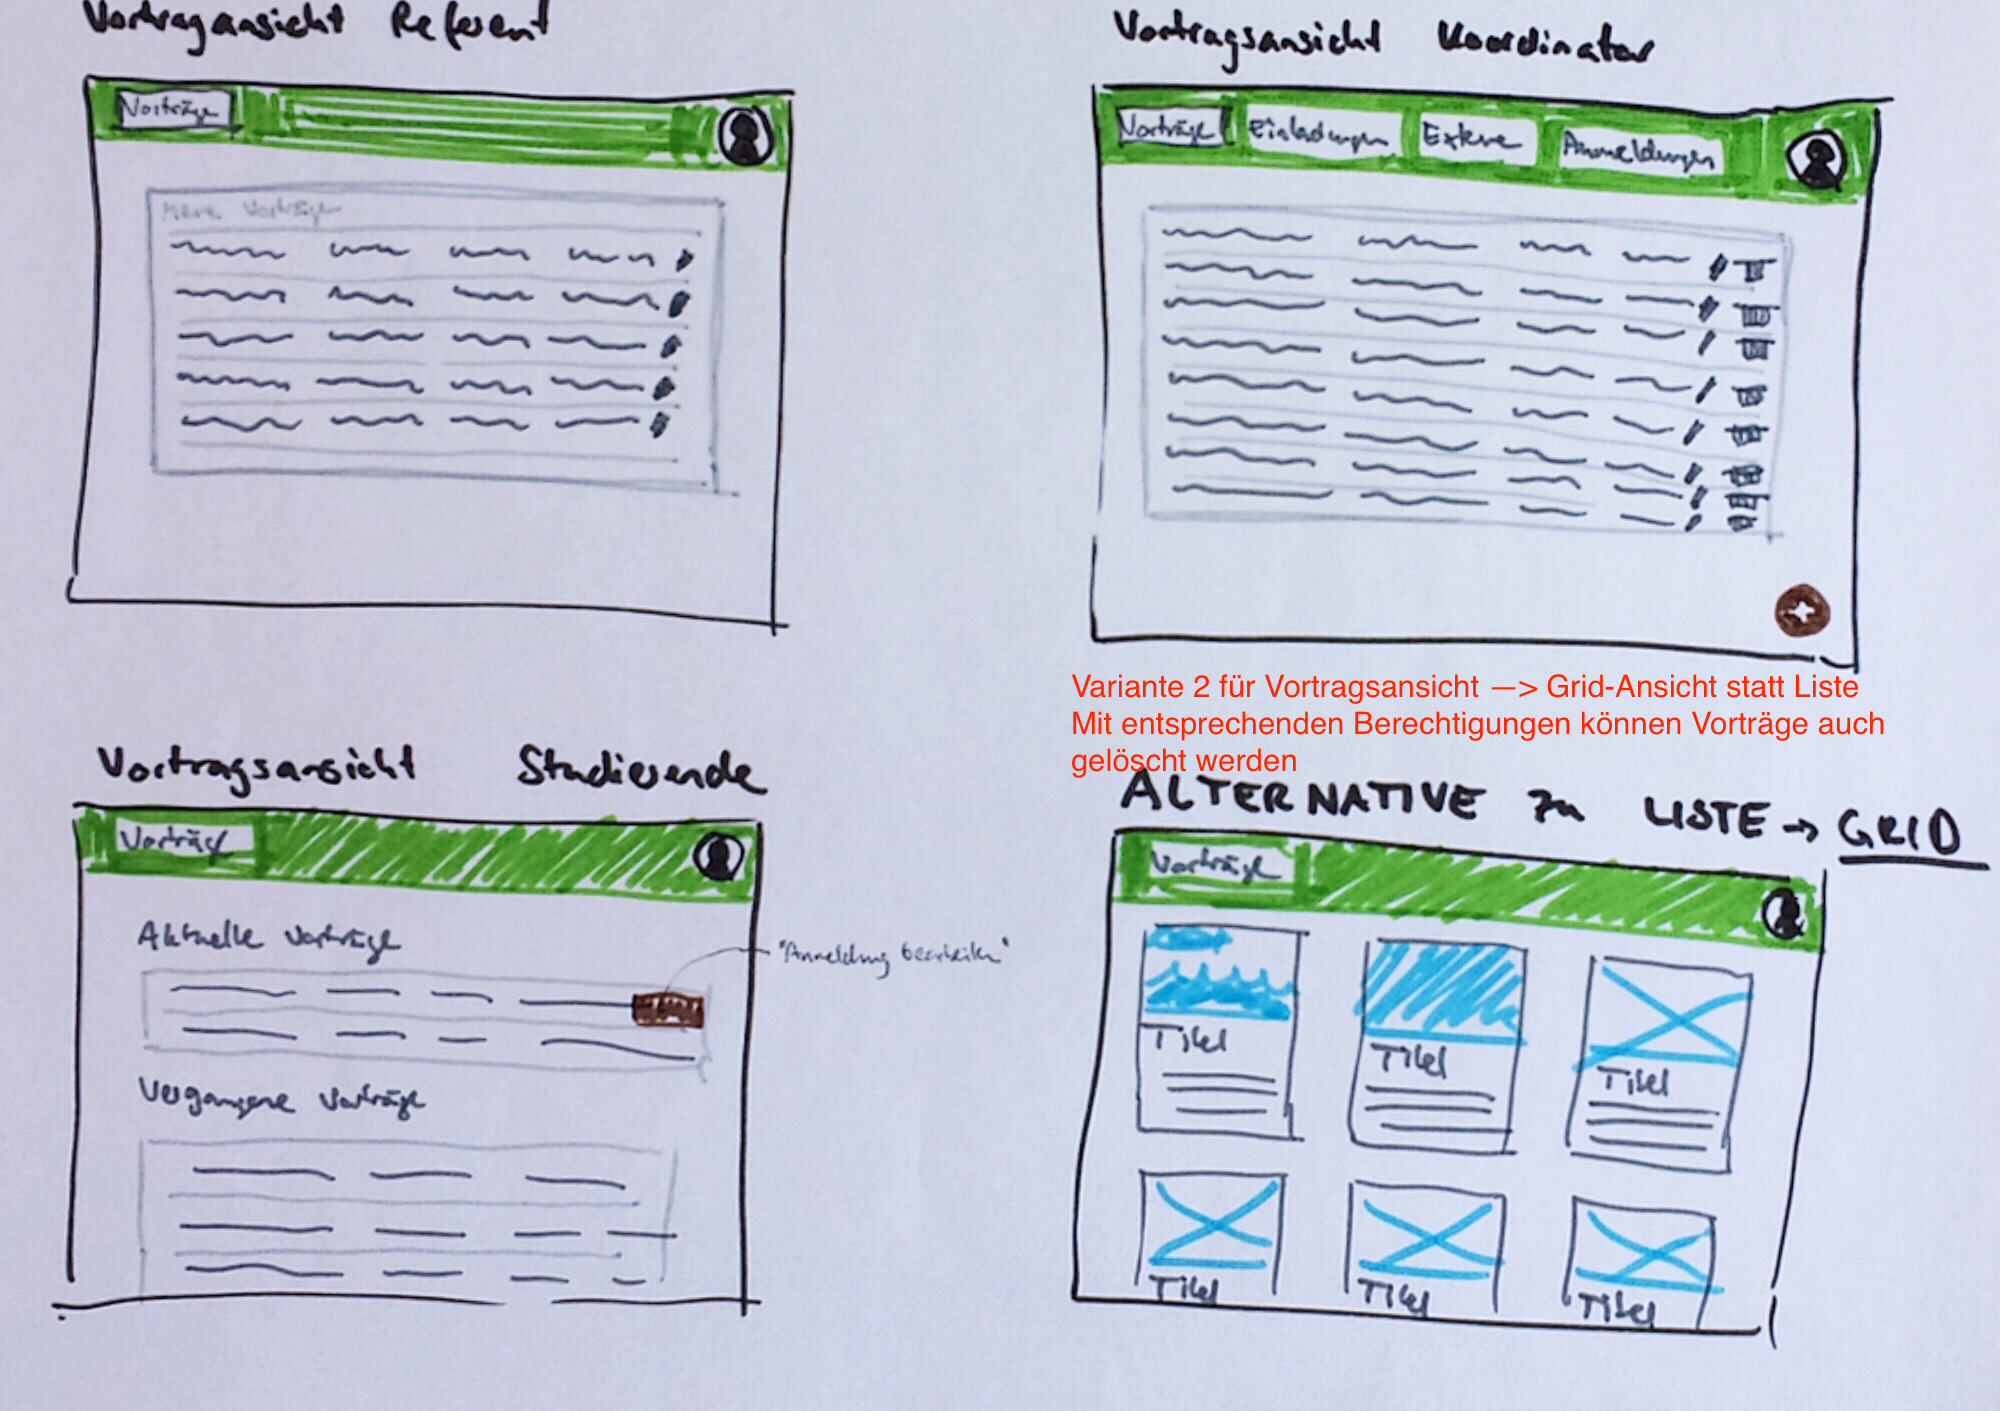
\includegraphics[width=0.8\textwidth]{prototyp/Vortragansicht}

\section{Architektur}
Unsere Implementation des "Event-Planners" wurde mit Microservices realisiert. Wir verwenden dazu "Eureka", eine Library entwickelt von Netflix https://github.com/netflix/eureka.  Unsere Applikation verwendet fünf Microservices, welche im nachfolgenden Abschnitt genauer beschrieben sind. Die Kommunikation zwischen den Microservices läuft über REST-APIs.

\subsection{Datenbank}
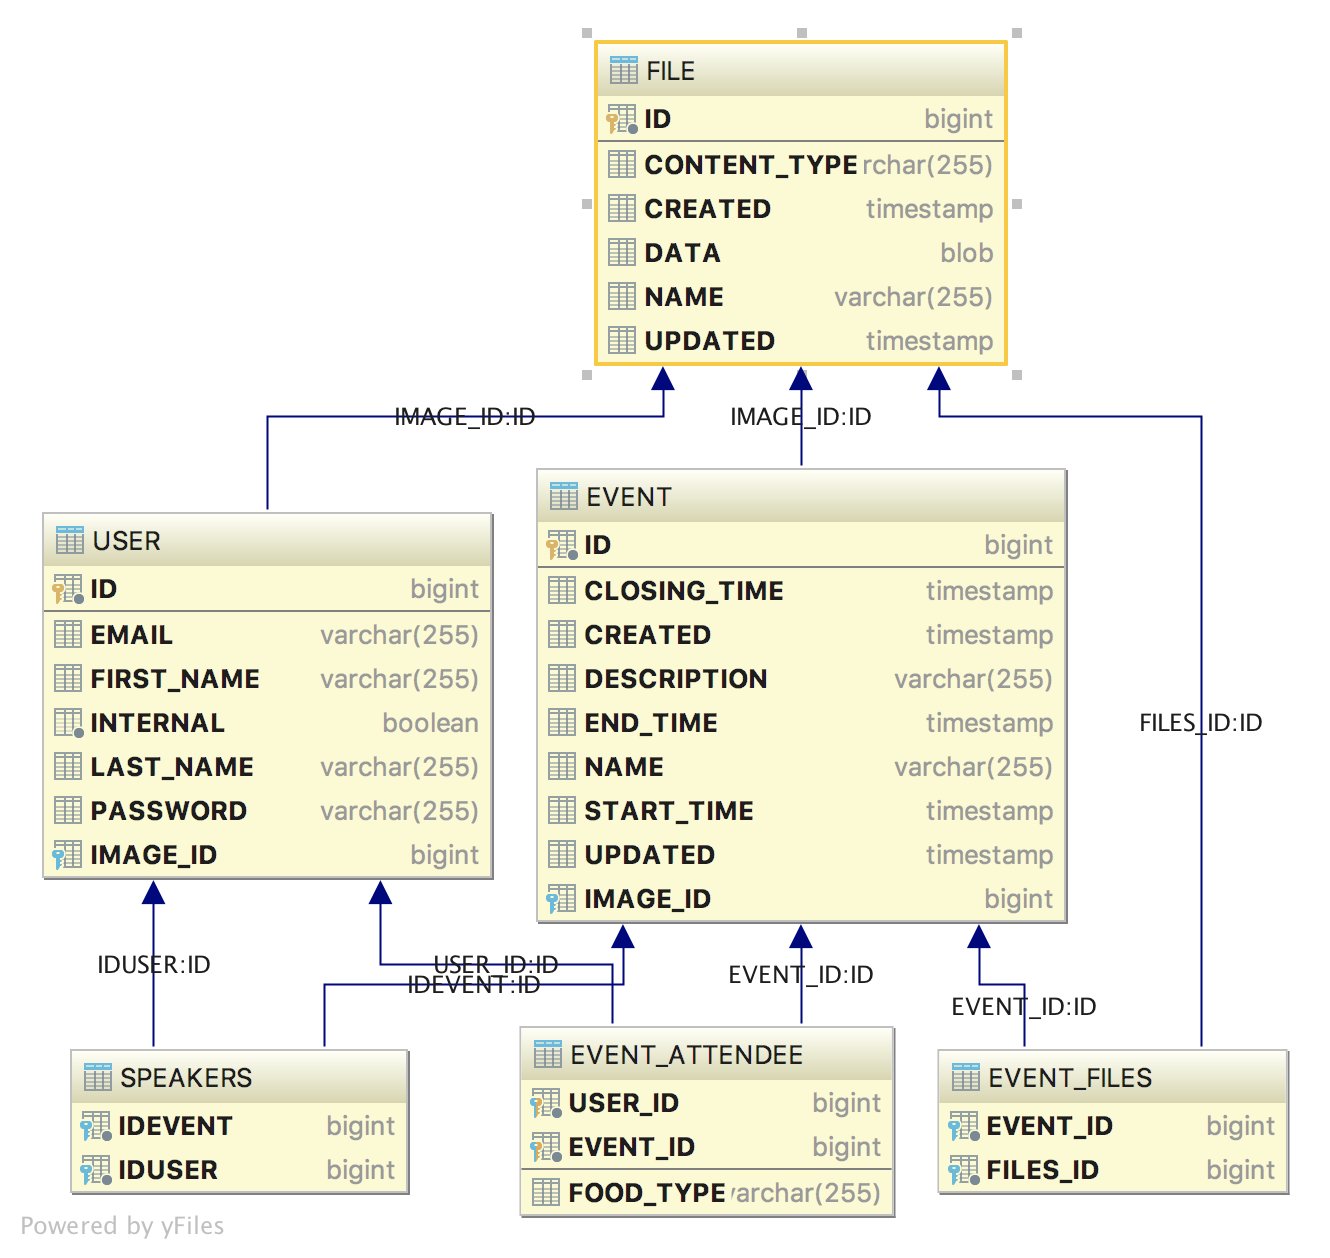
\includegraphics[width=1\textwidth]{dbSchema}

\subsection{Microservices}
\subsubsection{Registry}
	Das "Bindeglied" zwischen den verschiedenen Microservices. Die Microservices verbinden sich auf die Registry um dort die URIs der anderen Microservices zu bekommen. Dadurch wird es möglich, die Applikation auf mehreren Servern verteilt laufen zu lassen.

\subsubsection{Eventmanagement}
	Beinhaltet alle Entitäten sowie die Businesslogik unserer Applikation und stellt CRUD Operationen über eine REST-API zur Verfügung. Bestimmte Endpunkte sind dabei nur nach einer Authentifizierung und Autorisierung möglich.

\subsubsection{Frontend}
	Hostet die statischen Assets unserer Webseite und stellt sie über eine http/https Schnittstelle zur Verfügung. Die Webseite, welche mit Angular und Ionic erstellt wurde, ist eine Single Page App und lädt alle Daten asynchron vom eventmanagement service.

\subsubsection{Mailer}
	Ein sehr simpler Microservice der eine API zum Versenden von Mails bietet. Diese API kann nur mit einem Token angesprochen werden und ist nur für die Verwendung aus anderen Microservices angedacht. 

\subsubsection{Scheduler}
	Der Scheduler in bestimmten Intervallen oder zu bestimmten Zeiten Tasks aus. Ein Beispiel hierfür wäre, nicht verwendete (keine Referenz mehr) Mediadateien jede Nacht zu löschen. Hier wird auch geprüft, ob das Anmeldungsfenster eines Events geschlossen wurde und verschickt dann (über den "mailer" microservice" emails and alle Beteiligten.

\newpage

\begin{appendices}

\textbf{Github Repository}\\
https://github.com/lukeisontheroad/simple\_event\_planner\\
\\

\newpage

\end{appendices}

\end{document}
